\documentclass[12pt, a4paper]{article}
\usepackage[utf8]{inputenc}
\usepackage[margin=1.2in]{geometry}
\usepackage{multicol}
\usepackage{multirow}
\usepackage{url}
\usepackage{graphicx}
\usepackage{amsfonts}
\usepackage[tbtags]{amsmath}
\usepackage{amsfonts,amssymb,amsmath,graphicx,hyperref}
\usepackage{tikz}
\usetikzlibrary{arrows}
\usetikzlibrary{arrows.meta}
\usepackage{caption}
\usepackage{subcaption}
\usepackage{float}
\usepackage{algorithm}
\usepackage{algpseudocode}
\usetikzlibrary{shapes,arrows}

% Define the title and author data

\date{\vspace{-5ex}\today} % Position the date higher up

\begin{document}

% Start title page
\begin{titlepage}
    \centering
    \vspace*{1 cm}
    
    \textsc{\LARGE Lempel Ziv Welch Algorithm}\\[1.5 cm] % University name
    \textsc{\Large Bangladesh University of Engineering and Technology}\\[0.5 cm] % Department name
    \textsc{\large LaTex Report Submission On Presentation}\\[0.5 cm] % Report Type
    
    % Draw a line


    \rule{\linewidth}{0.2 mm} \\[1.5 cm]
    
    % Set the layout for the author information
    \begin{minipage}{0.4\textwidth}
        \begin{flushleft} \large
            \emph{Authors:}\\
            Munim Thahmid\\ % Author name
            H.M.Shadman Tabib\\ % Author name
            Tasriad Ahmed Tias
        \end{flushleft}
    \end{minipage}
    ~
    \begin{minipage}{0.4\textwidth}
        \begin{flushright} \large
            \emph{Student IDs:} \\
            2005097 \\ % Student ID
            2005103\\ % Student ID
            2005106
        \end{flushright}
    \end{minipage}\\[2 cm]
    
    % Date
{\large \today\vspace{2cm}}
    
    \vfill % Fill the rest of the page with whitespace
\end{titlepage}
% End title page

\pagenumbering{roman}
% The rest of your document contents follows here...
\tableofcontents
\newpage

\listoffigures

\listoftables
\newpage

\pagenumbering{arabic}
	%k=================================Tias==================================================== 
\section{Introduction}
This report briefly discusses the \textbf{Lempel–Ziv–Welch (LZW)} algorithm, a well-known universal lossless compression algorithm created by \textbf{Abraham Lempel}, \textbf{Jacob Ziv}, and \textbf{Terry Welch}. The algorithm is simple to implement and has the potential for very high throughput in hardware implementations.\cite{welch1984technique}
 It is the algorithm of the Unix file compression utility Compress and it's notably used in the GIF file format, favored for its ability to handle files of various sizes and noise levels. The dynamic or adaptive dictionary technique is a Type of data compression method that utilizes a dictionary or codebook to replace repetitive Patterns or strings of data with shorter codes. This technique can adapt to the characteristics of the input data, making it suitable for a wide range of applications.
\section{Adaptive Dictionary Techniques}
\textbf{LZW} is an adaptive compression algorithm that does not assume any prior knowledge of the symbol probabilities based on the work of Ziv and Lempel \textbf{LZ77} - Assumes patterns recur close together \textbf{LZ78} - Based on the entire previously coded sequence.\cite{ziv1977universal} LZW combines aspects of both \textbf{LZ77} and \textbf{LZ78} techniques, resulting in efficient data compression. The dynamic or adaptive dictionary technique, specifically LZ77, is a popular algorithm used for dictionary coding. This technique can compress data efficiently by utilizing a sliding window approach. The dynamic dictionary technique allows the dictionary or codebook to be updated dynamically as the encoding or decoding process progresses. This enables the technique to adapt to the specific patterns and structures present in the input data.
\subsection{LZW Encoding}
The encoding process of LZW involves building a dictionary of patterns encountered in the input data. As the encoding progresses, new patterns are added to the dictionary, resulting in shorter codes for repetitive sequences.
The dictionary is created while the data are being encoded. So encoding can be done on the fly. The dictionary need not be transmitted. The dictionary can be built up at the receiving end on the fly. If the dictionary overflows then we have to reinitialize the dictionary and add a bit to each one of the code words. Choosing a large dictionary size avoids overflow, but spoils compressions. A codebook or dictionary containing the source symbols is constructed. For 8-bit monochrome images, the first 256 words of the dictionary are assigned to the gray levels 0-255. The remaining part of the dictionary is filled with sequences of the gray levels.LZW compression works best when applied on monochrome images and text files that contain repetitive text/patterns.
\subsection{LZW Decoding}
The decoding process of LZW involves reconstructing the original data from the encoded codes. The decoder uses the dictionary to replace codes with their corresponding patterns
 \section{Compression Algorithm}
 %do not use math here,tias%
 A dictionary is initialized to contain the single-character strings corresponding to all the possible input characters (and nothing else except the clear and stop codes if they're being used). The algorithm works by scanning through the input string for successively longer substrings until it finds one that is not in the dictionary. When such a string is found, the index for the string less the last character (i.e., the longest substring that is in the dictionary) is retrieved from the dictionary and sent to the output, and the new string (including the last character) is added to the dictionary with the next available code. The last input character is then used as the next starting point to scan for substrings. In this way, successively longer strings are registered in the dictionary and made available for subsequent encoding as single output values. The algorithm works best on data with repeated patterns, so the initial parts of a message will see little compression. As the message grows, however, the compression ratio tends asymptotically to the maximum.
 \subsection{Pseudocode}
 \begin{algorithm}
\caption{LZW Compression Algorithm}
\begin{algorithmic}[1]
\Procedure{LZW\_COMP}{}
\State STRING = get input character
\While{there are still input characters}
    \State CHARACTER = get input character
    \If{STRING \& CHARACTER is in the S\_TABLE}
        \State STRING = STRING \& CHARACTER
    \Else
        \State output the codeword for STRING
        \State add STRING \& CHARACTER to S\_TABLE
        \State STRING = CHARACTER
    \EndIf
\EndWhile
\State output the codeword for STRING
\EndProcedure
\end{algorithmic}
\end{algorithm}
 \begin{figure}
    \centering
    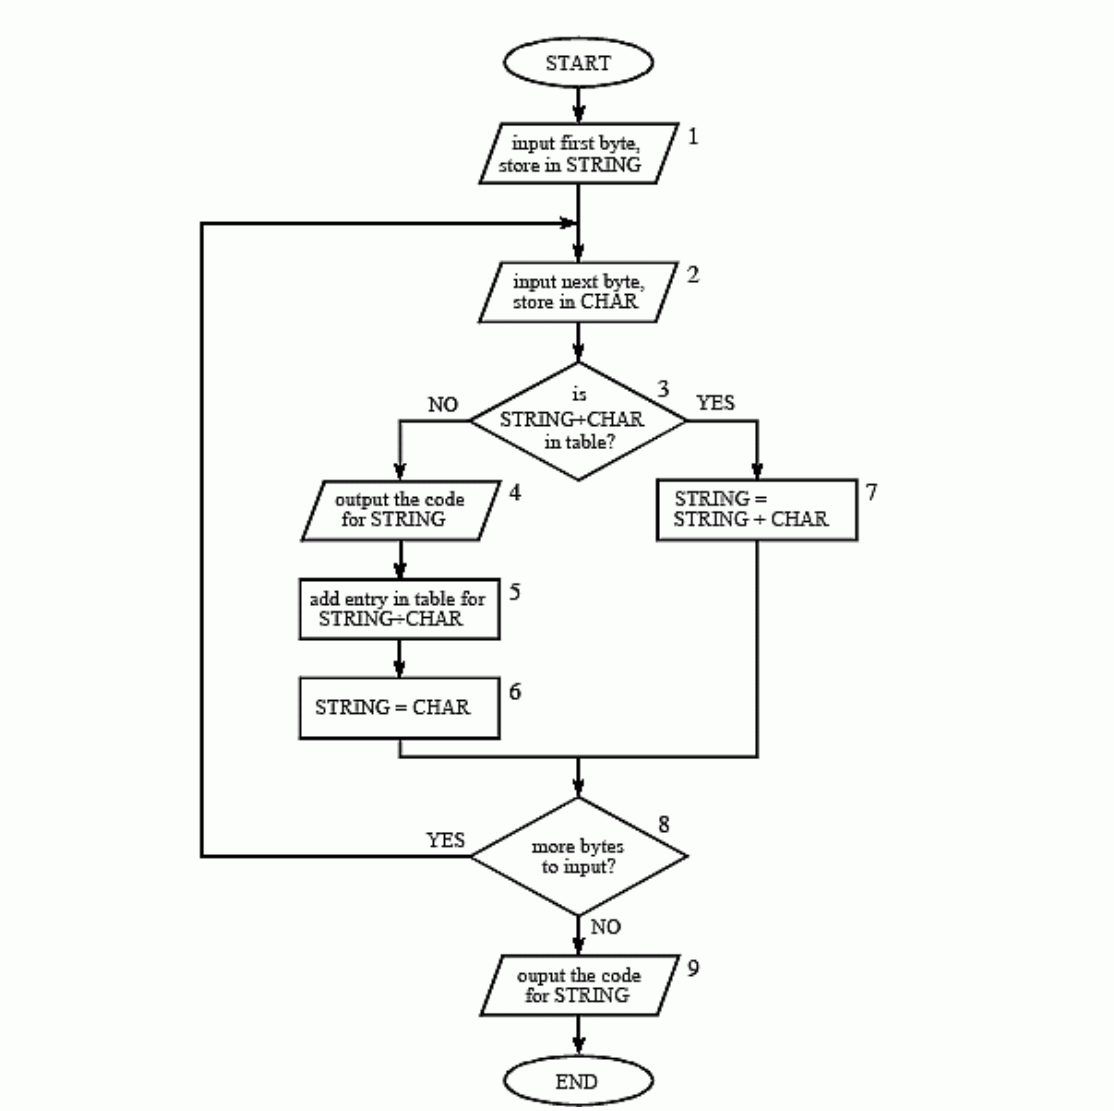
\includegraphics{images/compression.png}
    \caption{LZW Compression Flow Chart}
    \label{fig:enter-label}
\end{figure}
 \cite{smith1997scientist}
 \newpage
 \subsection{Illustrated Example}
 The compression procedure is as follows. It starts by
reading the first character in the source and assigning it to
STRING. The compression is then performed in the WHILE loop,
with a decision regarding the novelty of the current string made in the
IF-THEN-ELSE sequence. Each new character in the same string
is read at the beginning of the WILE loop and is assigned to
CHARACTER. If the previous STRING, concatenated with
CHARACTER is found in the S-TABLE then the compression
should continue by replacing the old STING with the new
concatenated one. This suing expansion process continues until a
a new character is encountered which makes the string a candidate for
entry into the S-TABLE. Now, a single code representing the old string of more than one character is output, while the new string is
placed into the S-TABLE. Finally, the last character in the new
string is assigned to STRING to start the next cycle of a string
buildup process. This process continues until the end-of-file
\textbf{\textless EOF\textgreater
} is encountered. \cite{kinsner1991lempel}
The compression algorithm uses two variables: CHAR and STRING. The variable, CHAR, holds a single character, i.e., a single byte value between 0 and 255. The variable, STRING, is a variable length string, i.e., a group of one or more characters, with each character being a single byte. In box 1 of Fig. 2, the program starts by taking the first byte from the input file and placing it in the variable, STRING. Fig. 2 shows this action in line 1. This is followed by the algorithm looping for each additional byte in the input file, controlled in the flow diagram by box 8. Each time a byte is read from the input file (box 2), it is stored in the variable, CHAR. The data table is then searched to determine if the concatenation of the two variables, STRING+CHAR, has already been assigned a code (box 3). If a match in the code table is not found, three actions are taken, as shown in boxes 4, 5 \& 6. In box 4, the 12-bit code corresponding to the contents of the variable, STRING, is written to the compressed file. In box 5, a new code is created in the table for the concatenation of STRING+CHAR. In box 6, the variable, STRING, takes the value of the variable, CHAR. An example of these actions is shown in lines 2 through 10 in Fig. 2, for the first 10 bytes of the example file.
When a match in the code table is found (box 3), the concatenation of STRING+CHAR is stored in the variable, STRING, without any other action taking place (box 7). That is, if a matching sequence is found in the table, no action should be taken before determining if there is a longer matching sequence also in the table. An example of this is shown in line 11, where the sequence: STRING+CHAR = in, is identified as already having a code in the table. In line 12, the next character from the input file, /, is added to the sequence, and the code table is searched for: in/. Since this longer sequence is not in the table, the program adds it to the table, outputs the code for the shorter sequence that is in the table (code 262), and starts over searching for sequences beginning with the character, /. This flow of events is continued until there are no more characters in the input file. The program is wrapped up with the code corresponding to the current value of STRING being written to the compressed file (as illustrated in box 9 of Fig. 2 and line 45).
\begin{figure}
    \centering
    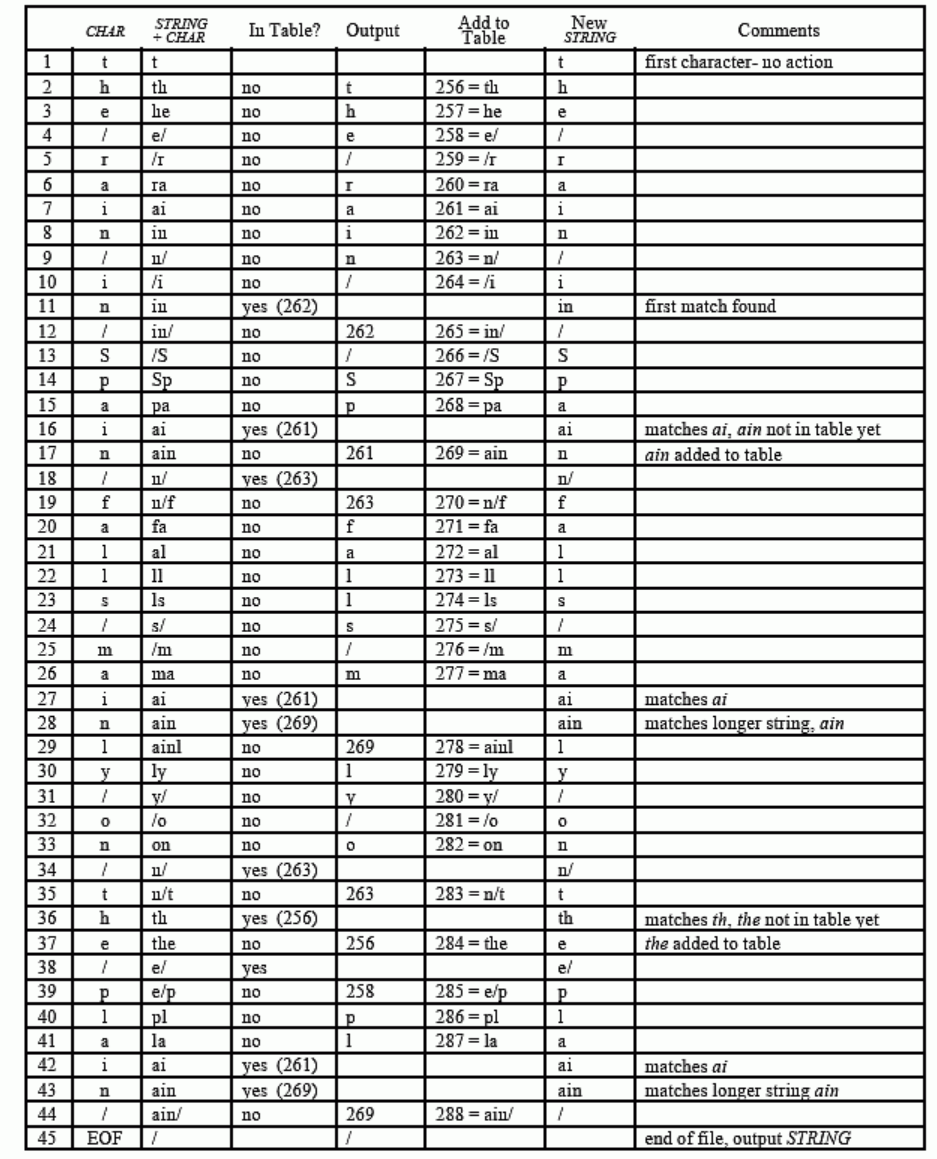
\includegraphics{images/example.png}
    \caption{Illustrated example of compression procedure. This shows compression of the phrase: the/rain/in/Spain/falls/mainly/on/the/plain/.}
    \label{fig:enter-label}
\end{figure}
 \newpage
 %-------------Tabib-----------%
\section{Behavioral Study of Data Structures On Lempel-Ziv-Welch (LZW) Data Compression Algorithm And Its Computational Complexity}

This study explores the LZW data compression algorithm, focusing on the linear array with linear search implementation for dictionary management. The LZW algorithm, widely used for compressing text and monochrome images, relies on a dictionary-based approach, where the efficiency of dictionary operations—insertion and search—is crucial for performance.

In a linear array implementation, dictionary searches are performed sequentially from the lower to the upper bound, returning a boolean value based on the presence of the string plus character (`STRING+CHAR`) combination. If not found, the dictionary is updated with this combination as the topmost element, and its size is incremented to accommodate the new entry. This approach, while straightforward, leads to an average computational complexity of $O(n^2)$ for dictionary updates, where $n$ is the length of the input sequence.

\textbf{Theorem 1.} The linear array with linear search implementation for the LZW algorithm has a computational complexity of $O\left(\frac{n(n+1)}{2}\right)$ for dictionary updates, where $n$ is the length of the input sequence.

\textbf{Proof.} Considering each unsuccessful search results in a dictionary size increment, the total number of operations for inserting all elements is the sum of an arithmetic sequence, leading to $O\left(\frac{n(n+1)}{2}\right)$.

Despite its simplicity, this method suffers from scalability issues for large datasets due to its quadratic growth in computational complexity. Future work may involve optimizing dictionary management or exploring alternative data structures to enhance compression efficiency and reduce computational overhead.
In LZW compression utilizing a linear array, dictionary searches proceed in a sequential manner from the beginning to the end of the array. The computational complexity associated with this method stems from the progressive growth of the dictionary as new `STRING+CHAR` combinations are appended.


The average computational complexity of updating the dictionary in the linear array-based LZW compression algorithm is \( O\left(\frac{N(N + 1)}{4}\right) \), with \( N \) denoting the number of input symbols.


\begin{proof}
For each unsuccessful search, the dictionary expands, increasing the search space linearly. The average number of comparisons per insert operation thus corresponds to the mean of the first \( N \) natural numbers, which yields the complexity:
\begin{align*}
    |X| & = |X|\left(\frac{1}{N} \sum_{i=1}^{N} i \right) \\
    & = |X|\left(\frac{1}{N} \frac{N(N + 1)}{2}\right) \\
    & = |X|\left(\frac{N + 1}{2}\right) \\
    & = |X|\left(\frac{N}{2} + \frac{1}{2}\right) \\
    & = |X|\left(\frac{N + 3}{4}\right) \text{ for large } N.
\end{align*}
This reflects the quadratic growth in time complexity concerning the number of inputs due to the linear search algorithm in a linear array data structure.
\end{proof}


\textbf{LZW Decompression Linear Array Implementation with Linear Search}

Decompression in LZW with a linear array applies a straightforward approach. It involves checking the availability of the New Code translation in the dictionary. If the translation is unavailable, the New Code is appended after the current maximum index, which leads to a simple and computationally efficient decompression since it only requires one comparison per input symbol to check for the existence of the New Code in the dictionary.

\begin{theorem}
The linear array implementation of LZW decompression operates with a computational complexity of \( O(|C|) \).
\end{theorem}

\begin{proof}
Given that decompression entails a single lookup for translating the New Code and appending it if absent, the time complexity is constant for each symbol:

\begin{align*}
|C| \cdot \left( 1 \times \frac{1}{n} \sum_{i=1}^{n} 1 \right) &= |C| \cdot \left( \frac{1}{n} \times n \right) \\
&= |C| \cdot 1 \\
&= O(|C|).
\end{align*}

Thus, the linear array implementation for LZW decompression does not inherently require improvements for computational cost reduction, as it already operates at optimal efficiency.\\
\end{proof}

\textbf{Binary Search Tree (BST) Implementation of LZW}

The BST approach in LZW enhances the search and update operations of the dictionary. It uses a binary tree structure for efficient insertions and lookups, significantly reducing the time complexity for these operations. During each compression cycle, the algorithm checks for the `STRING+CHAR` pattern in the BST dictionary, and if not found, it proceeds to insert a new node with this value.

\begin{theorem}
The BST-based LZW compression algorithm achieves a computational complexity of \( O(X \cdot (\log (N^\frac{1}{N}))) \), where \( X \) is the length of the input sequence and \( N \) is the number of unique input symbols.
\end{theorem}

\begin{theorem}
The BST implemented LZW compression algorithm takes \( O(X \cdot \log (N^{\frac{1}{N}})) \) time, where \( X \) is the length of the sequence and \( N \) is the number of nodes in the BST.
\end{theorem}

\begin{proof}
Considering a binary search tree (BST) utilized in the LZW compression, we acknowledge two possibilities during its construction: a successful search and an unsuccessful search. The average case time complexity for a search operation in a BST with \( N \) elements is \( O(\log N) \). Thus, we consider the average of successful and unsuccessful search operations, giving us the following:
\begin{align*}
O(\log(N) + O(\log(N))) &= O\left(\frac{2 \cdot \log(N)}{2}\right) \\
&= O(\log(N)).
\end{align*}

As the number of nodes \( N \) increases with each insertion, we have to consider the size of the BST at each point of insertion. If \( n_i \) denotes the number of nodes after the \( i^{th} \) insertion, the time complexity for a search is \( O(\log(n_i)) \). Consequently, the average comparison time for \( N \) insertions is:
\begin{align*}
\frac{1}{N} (O(\log(n_1) + O(\log(n_2)) + \dots + O(\log(n_N)))) &= O\left(\frac{1}{N} \sum_{i=1}^{N} \log(n_i)\right) \\
&= O\left(\log\left(n_1 \cdot n_2 \cdot \ldots \cdot n_N\right)^{\frac{1}{N}}\right) \\
&= O\left(\log\left(N!\right)^{\frac{1}{N}}\right).
\end{align*}

Assuming that the BST operations are distributed evenly among \( N \) nodes, the comparison time to compress the entire sequence \( X \) can be given by:
\begin{align*}
O(X \cdot \log(N!^{\frac{1}{N}})) &= O(X \cdot (\log(N!))^{\frac{1}{N}}) \\
&= O\left(X \cdot \left(\log\left(\prod_{i=1}^{N} i\right)\right)^{\frac{1}{N}}\right) \\
&= O(X \cdot (\log (N^{\frac{1}{N}}))).\\
\end{align*}
\end{proof}
\textbf{ Chained Hash table based Compression of LZW Algorithm}
\\
The chained hash table approach introduces hashing to improve the search and update efficiency in the LZW compression dictionary. This method hashes each `STRING+CHAR` combination, then either confirms its presence or inserts it into a linked list at the hashed index, which substantially improves the time complexity compared to the linear array and BST implementations.

\begin{theorem}
The average expected time for LZW compression with a chained hash table is \( O(X \cdot (1 + \text{AM}_{\alpha})) \), where \( X \) is the sequence length, and \( \text{AM}_{\alpha} \) is the average number of probes in a successful search.
\end{theorem}

\begin{proof}
Assuming an average load factor \( \alpha \) after each insertion into the dictionary, the time complexity can be expressed as an average of the successful and unsuccessful searches:
\begin{align*}
\frac{(1 + \alpha) + (1 + \alpha)}{2} &= 1 + \alpha.
\end{align*}

The load factor \( \alpha \) is dynamic and changes after each insertion. If \( a_i \) represents the load factor after the \( i^{th} \) insertion, then the average time complexity across \( n \) insertions is:
\begin{align*}
\frac{(1 + a_1) + (1 + a_2) + \ldots + (1 + a_n)}{n} &= 1 + \frac{\sum_{i=1}^{n} a_i}{n} \\
&= 1 + \text{AM}_{\alpha},
\end{align*}
where \( \text{AM}_{\alpha} \) is the arithmetic mean of the load factors after each insertion. Thus, the time complexity to compress the entire sequence \( X \) is given by:
\[
O(X \cdot (1 + \text{AM}_{\alpha})).
\]
\end{proof}
 \section{Anomalies In LZW With Relevant Example}
\begin{verbatim}
INPUT DATA STREAM: 01000101110010100101
\end{verbatim}

\begin{table}[h!]
\centering
\begin{tabular}{@{}cccccccccc@{}}
\toprule
\textbf{Position} & 1 & 2 & 3 & 4 & 5 & 6 & 7 & 8 & 9 \\ \midrule
\textbf{Subseq.} & 0 & 1 & 00 & 01 & 01 & 10 & 010 & 100 & 101 \\
\textbf{Num. Rep.} & $-$ & $-$ & 1 & 2 & 2 & 1 & 4 & 6 & 2 \\
\textbf{Bin. Encoded} & 0 & 1 & 0010 & 0011 & 1001 & 0100 & 1000 & 1100 & 101 \\ \bottomrule
\end{tabular}
\caption{Example of LZW Compression Encoding}
\label{tab:lzw_example}
\end{table}

\paragraph{Analysis of Encoding Size}
The LZW algorithm is designed to take advantage of redundancy in the input data stream for compression. In the provided binary sequence, the LZW encoding process assigns a new binary code to each unique sequence encountered, resulting in an initial dictionary build-up phase where encoded blocks may appear larger than the original data. This phenomenon is evident in the numerical representation of the sequence, where consecutive patterns are assigned incrementally larger binary codes.

\paragraph{Optimal Conditions for LZW}
LZW compression is most effective with large and redundant data sets. The algorithm progressively builds a dictionary of input sequences, which allows it to efficiently encode repeated sequences as the data stream progresses. However, for non-redundant and short data sets, LZW may not only fail to reduce the size but can actually increase it due to the overhead of the dictionary encoding. This overhead is necessary to ensure that the decompression process can accurately reconstruct the original data.

%-----------Munim-------%
\section{Decoding}

Decoding in LZW serves as the reverse process of compression. While compression reduces the size of data by replacing repeated patterns with codes, decoding reconstructs the original data from these codes. It plays a crucial role in applications where compressed data needs to be decompressed for analysis, transmission, or storage.\cite{liu2012survey}

\subsection{Decoding Process Overview}

The decoding process in LZW involves reconstructing the original data stream from the compressed representation generated during the encoding phase. It relies on a dictionary that maps codes to sequences of symbols. As each code corresponds to a unique symbol sequence, decoding involves translating the codes back into their original sequences. \cite{shannon1948mathematical}

\subsection{Decoding Algorithm}

The decoding algorithm\cite{hoffman1970adaptive} in LZW is systematic and straightforward. It follows a step-by-step process to reconstruct the original data stream from the compressed data:

\begin{enumerate}
    \item \textbf{Initialize Dictionary:} Begin by initializing the dictionary with the same initial entries used during the encoding phase. This ensures consistency between the encoding and decoding processes.
    \item \textbf{Read Compressed Data:} Read the compressed data stream containing the encoded symbols generated during compression.
    \item \textbf{Decode Symbols:} Process the encoded symbols one by one and reconstruct the original data stream:
    \begin{enumerate}
        \item If the current code exists in the dictionary, retrieve the corresponding symbol sequence.
        \item If the current code is not found in the dictionary, create a new entry by concatenating the symbol sequence of the previous code with the first symbol of the previous code.
        \item Output the decoded symbol sequence.
        \item Update the dictionary with the new entry for the current code.
        \item Update the previous code variable with the value of the current code for the next iteration.
    \end{enumerate}
    \item \textbf{Continue Decoding:} Repeat the decoding process until all encoded symbols in the data stream have been processed.
\end{enumerate}
\pagebreak
\subsection{Pseudocode for Decoding}

The decoding algorithm can be summarized in pseudocode as follows:

\begin{algorithm}[H]
\SetAlgoLined
\KwData{Compressed data stream}
\KwResult{Decoded original data}
 Initialize decoder dictionary with initial entries from encoding phase\;
 Read compressed data stream\;
 Initialize variables: previousCode, currentCode, decodedOutput\;
 \While{there are encoded symbols to decode}{
    Read next encoded symbol from the compressed data stream\;
    \If{currentCode exists in the dictionary}{
        Retrieve symbol sequence corresponding to currentCode\;
    }
    \Else{
        Create new dictionary entry for currentCode by concatenating symbol sequence of previousCode with first symbol of previousCode\;
    }
    Output decoded symbol sequence\;
    Update dictionary with new entry for currentCode\;
    Update previousCode to currentCode\;
 }
 \caption{LZW Decoding Algorithm}
\end{algorithm}


\clearpage % Start a new page for clarity in the document

\section{Application}

The Lempel-Ziv-Welch (LZW) data compression algorithm finds applications in various domains due to its effectiveness in reducing the size of data while preserving its integrity. Some notable applications include:

% Define block styles
\tikzstyle{startstop} = [rectangle, rounded corners, minimum width=3cm, minimum height=1cm, text centered, draw=black, fill=red!30]
\tikzstyle{io} = [trapezium, trapezium left angle=70, trapezium right angle=110, minimum width=3cm, minimum height=1cm, text centered, draw=black, fill=blue!30]
\tikzstyle{process} = [rectangle, minimum width=3cm, minimum height=1cm, text centered, draw=black, fill=orange!30]
\tikzstyle{arrow} = [thick,->,>=stealth]

\subsection{Text Compression}

One of the primary applications of LZW is in compressing textual data. Text files often contain repetitive patterns and sequences, making them suitable candidates for compression using LZW. By encoding repeated substrings with shorter codes, LZW significantly reduces the storage space required for text documents, making them easier to store and transmit over networks.

\subsubsection{Illustration of Text Compression using LZW}

\begin{figure}[htbp]
    \centering
    \begin{tikzpicture}[node distance=2cm, auto]
        % Nodes
        \node (input) [startstop] {Text Input};
        \node (compressor) [process, right of=input, xshift=2cm] {LZW Compressor};
        \node (compressed) [io, right of=compressor, xshift=3cm] {Compressed Text};
        \node (decompressor) [process, below of=compressor] {LZW Decompressor};
        \node (output) [startstop, below of=decompressor] {Decompressed Text};
        
        % Arrows
        \draw [arrow] (input) -- (compressor);
        \draw [arrow] (compressor) -- (compressed);
        \draw [arrow] (compressed) |- (decompressor);
        \draw [arrow] (decompressor) -- (output);
    \end{tikzpicture}
    \caption{Illustration of Text Compression using LZW Algorithm}
    \label{fig:lzw_text_compression}
\end{figure}

In Figure \ref{fig:lzw_text_compression}, we illustrate the process of text compression using the LZW algorithm. The input text undergoes compression using the LZW compressor, resulting in a compressed text representation. This compressed text can then be decompressed using the LZW decompressor to retrieve the original text data.
.\cite{mackay2003information}

\subsection{Image Compression}

LZW is also used in image compression algorithms, particularly in monochrome or grayscale images. Similar to text data, images often contain repeated patterns, especially in areas of uniform color or texture. By identifying and encoding these patterns efficiently, LZW-based compression techniques can significantly reduce the size of image files without perceptible loss in quality.\cite{bloom1970space}

\subsection{Network Communication}

In network communication protocols, where bandwidth and data transmission speed are crucial factors, LZW compression plays a vital role in optimizing data transfer. By compressing data packets before transmission and decompressing them at the receiving end, LZW helps reduce network congestion and latency, thereby improving overall network performance.

\subsection{File Archiving and Compression Utilities}

Many file archiving and compression utilities, such as ZIP, GZIP, and TAR, employ LZW-based algorithms to compress multiple files and directories into a single archive file. These utilities use LZW to compress individual files before packaging them into the archive, allowing users to save disk space and streamline file management tasks.

\subsection{Embedded Systems and IoT Devices}

In resource-constrained environments, such as embedded systems and Internet of Things (IoT) devices, efficient data storage and transmission are critical requirements. LZW's lightweight implementation and ability to compress data in real-time make it suitable for use in these systems, enabling developers to optimize memory usage and enhance device performance.

Overall, the versatility and effectiveness of the LZW algorithm make it a widely adopted solution across various applications, contributing to improved data management, communication efficiency, and resource utilization in diverse domains.

\section{Conclusion and Future Enhancement}

The LZW (Lempel-Ziv-Welch) algorithm, a cornerstone in data compression, has seen significant improvements and enhancements since its inception. These developments have aimed to augment the compression ratio and diminish computational complexity. In this context, the paper presented an empirical and theoretical evaluation of various data structure implementations within the LZW framework, namely linear arrays, binary search trees (BST), and chained hash tables.There are already significant works regarding variable rate coding using LZW algorithm.\cite{ZivLempel1978}   

    
    


The current findings indicate that while the chained hash table implementation outperforms linear arrays and BSTs in encoding, for decoding, the simpler linear array method proves more efficient, almost eliminating the need for further optimization in terms of computational expense. However, to adapt LZW compression to a wider range of applications and enhance its effectiveness, several avenues for future work emerge:

\begin{itemize}
  \item \textbf{Authentication of Compression Techniques:} Future studies could focus on integrating authentication mechanisms within the LZW algorithm to ensure data integrity and security during compression, especially for applications in sensitive data transmission.
  \item \textbf{Adaptive Dictionary Management:} Developing adaptive strategies for dictionary management that can dynamically adjust based on the nature of the data being compressed, to better exploit redundancy patterns and improve compression rates.
  \item \textbf{Parallel Processing:} Exploiting modern multi-core and parallel processing technologies to improve the speed of LZW operations, particularly for large data sets where current implementations may be less efficient.
  \item \textbf{Algorithmic Improvements:} Investigating enhancements to the core algorithm that might reduce the computational overhead or improve compression without compromising decompression accuracy.
  \item \textbf{Hybrid Compression Techniques:} Combining LZW with other compression methods, such as arithmetic coding, to potentially yield better compression ratios and adaptability across various data types.
\end{itemize}

These potential research directions could further the capabilities of the LZW algorithm, ensuring its continued relevance and efficiency in the field of data compression
\bibliographystyle{plain}
\bibliography{references}
    
\end{document}
